\documentclass[12pt,twoside,titlepage]{ingenius}
\usepackage[figuresright]{rotating}
\usepackage{algorithmic}
\usepackage{algorithm}
\usepackage{units}
\usepackage{dblfloatfix}
\usepackage{amssymb}
\usepackage{caption}
\usepackage{subcaption}
\usepackage{bm}
%\usepackage{mathpazo}
%\renewcommand{\familydefault}{\rmdefault}
%\usepackage{times}
%\usepackage{helvetica}
%\renewcommand{\familydefault}{\sfdefault}
%\usepackage{newcent}
%\usepackage{chancery}
%\usepackage{fourier}
%\usepackage{beraserif}
%\usepackage{mathpazo}
\usepackage{textcomp}
\usepackage{pifont}
\usepackage{cite}
\usepackage{xcolor,colortbl}
\usepackage{amsmath}
\usepackage{upgreek}


\titulo{Análisis de Imágenes Rayos X Cerebrales Usando Redes Neuronales Convolucionales VGGNet}
\tituloa{Brain X-ray Image Analysis Using VGGNet Convolutional Neural Networks}


\autores{PhD. Angel Cuenca $^{1}$, Ing. Edgar Basurto $^{2}$, Ing. Rafael Larrea$^{3}$}

\adscripcionautor{%
$^{1}$Facultad de Ciencias Matemáticas y Físicas, Universidad de Guayaquil - Ecuador.\\
$^{2}$Investigador Independiente - edabaro0191@gmail.com.\\
$^{3}$Investigador Independiente - rlarrea@gmail.com}


%% Datos para adcripcion
\fechar{01-11-2016}%Fecha recibido 
\fechaa{27-12-2016}%Fecha aprovacion 
\autorad{Luna, M.; Moya, J.; Aguilar, W.; Abad, V.}%nombres adscripcion
\ano{2017} %Año
\mes{Enero-Junio}%Mes
\numero{17}%Numero de la revista que va a la adscripcion
\pag{67-72}%paginas

%%Datos para referencias
\newcommand{\apellido}{Cuenca A., Basurto E., Larrea R.}% Apellido o apellidos para referencia 
\newcommand{\titu}{Análisis de Imágenes Rayos X Cerebrales Usando CNN VGGNet}%titulo a la ref\erencia
%\newcommand{\mest}{}%mes de publicacion de revista
%\newcommand{\anoc}{}% año revista
%\newcommand{\revista}{}%nombre revista
%\newcommand{\num}{}%numero revista
\newcommand{\tipo}{Art\'iculo Cient\'if{}ico / Scientif{}ic Paper}%tipo de documento Punto de vista/Point of view,  Art\'iculo Cient\'if{}ico / Scientif{}ic Paper, Rese\~na bibliogr\'afica/Review


%%Datos para propiedades del pdf
\newcommand{\autor}{}%autor para propiedades del pdf
\newcommand{\pc}{}%palabras clave para propiedades del pdf
\newcommand{\kw}{}%keywords para propiedades del pdf

\usepackage{xcolor}
\usepackage{color}
\usepackage{titlesec}
\usepackage[spanish,english]{babel}
\titleformat{\section}
{\large \bfseries }
{\thesection.}{.5em}{}

\titleformat{\subsection}
{\normalsize \bfseries  }
{\thesubsection.}{.5em}{}

\titleformat{\subsubsection}
{\normalsize \bfseries }
{\thesubsubsection.}{.5em}{}

\usepackage{fancyhdr}
\pagestyle{fancy}
\fancyhf{}
\fancyhead[LO]{} % En las páginas impares, parte izquierda del encabezado, aparecerá el nombre de capítulo
%\fancyhead[RE]{{\rule[-2ex]{0pt}{3ex} \bf \revista} N.$^\circ$ \num, \mest \, de \anoc} % En las páginas pares, parte derecha del encabezado, aparecerá el nombre de sección
\fancyhead[LE,RO]{ \large \thepage  } % Números de página en las esquinas de los encabezados
\fancyhead[LO]{\rule[-2ex]{0pt}{3ex} {\it \apellido \,/ \titu}} % Números de página en las esquinas de los encabezados
%\fancyfoot[LE,RO]{\thepage} %Escribo este texto a la izquierda en las páginas impares y a la derecha en las pares
%\fancyfoot[LO,RE]{ \rule{300pt}{0.5pt}\\ \textsc{Ingenius}, {\it  Revista de Ciencia y Tecnolog\'ia.}\\ \copyright  \, 2013, {Universidad Polit\'ecnica Salesiana, Ecuador.}} %Escribo este texto a la izquierda en las páginas impares y a la derecha en las pares
%\fancyfoot[LO,RE]{\textsc{Ingenius}, {\it  Revista de Ciencia y Tecnolog\'ia}, 7(1) 2012: 1-6. \\ \copyright  \, 2012, {Universidad Polit\'ecnica Salesiana, Ecuador.}} %Escribo este texto a la izquierda en las páginas impares y a la derecha en las pares
\renewcommand{\headrulewidth}{0.5pt}
%\renewcommand{\footrulewidth}{0.5pt}

\usepackage[]{hyperref}
\hypersetup{
    pdftitle={\titu},
    pdfauthor={\autor},
    pdfsubject={Ingenius -- Revista de Ciencia y Tecnolog\'ia},
    pdfkeywords={\pc; \kw},
    pdfborder={0 0 0},
    bookmarks=true,
pdfstartpage=1,
pdfproducer=pdf\TeX{}-1.40.13. Andr\'es Sarmiento C.
}

\usepackage{xcolor}
\usepackage{color}
\usepackage{listings}%% lista de códigos
\usepackage{tikz}
%\input{config_c}

\usepackage{listings}%% lista de códigos
	\lstset{ 
		linewidth=0.5\textwidth,
		frame=tb,	
		%framerule=0.5pt,
		aboveskip=0.5cm,%Distancia Texto al codigo
		%framextopmargin=3pt,%Distancia Primera Linea-Borde Superior
		framexbottommargin=3pt,%Distancia Ultima Linea-Borde Inferior
		%framexleftmargin=0.4cm,%Distancia Borde Izquierdo Codigo-Borde Izquierdo Pagina
		framesep=0pt,
		rulesep=.8pt,%Espesor linea junto a los numeros
		backgroundcolor=\color{gray!10},
                     numbersep=5pt,
                     xleftmargin=3pt,
                     xrightmargin=8.5pt,
                     framextopmargin=10pt,
		rulesepcolor=\color{black},
		stringstyle=\ttfamily,
		floatplacement=htb,
		boxpos={c},
		breaklines=true,
		breakatwhitespace=true,
		showstringspaces = false,
		basicstyle=\small\ttfamily,
		commentstyle=\color{gray!45},
		keywordstyle=\bfseries,
		%linewidth=0.8\textwidth,
		title=\lstname,
		%numbers=right,%Posicion de los Numeros left=izquierda; right=derecha
		%numbersep=15pt, %separacion de numero 1,2,3,4 hacia el frame
		numberstyle=\tiny,
		numberfirstline = false,
		breaklines=true,
		}

	\lstnewenvironment{listing}[1][]
		{\lstset{#1}\pagebreak[0]}{\pagebreak[0]}
		\lstdefinestyle{consola}
		{basicstyle=\scriptsize\bf\ttfamily,
		 backgroundcolor=\color{gray75},
		}
	\lstdefinestyle{C}
		{language=C,
}


\newenvironment{tabla}
  {\par\bigskip\noindent\minipage{\linewidth}}
  {\endminipage\par\bigskip}

\newenvironment{figura}
  {\par\bigskip\noindent\minipage{\linewidth}}
  {\endminipage\par\bigskip}

\newenvironment{seudo}
  {\par\noindent\minipage{\linewidth}}
  {\endminipage\par\bigskip}

\begin{document}
\renewcommand{\lstlistingname}{Algorithm}
\setcounter{page}{1}
\renewcommand{\refname}{Referencia}
\renewcommand{\figurename}{Figura}
\renewcommand{\tablename}{Tabla}
\frenchspacing




\hyphenation{pro-pie-ta-rios co-ti-dia-na apro-xi-ma-da-men-te des-cri-be M\'e-xi-co co-ne-xi\'on ges-tio-na-das- r\'a-pi-da vi-sua-li-za-ción confi-gu-ra-cio-nes si-guien-tes va-rios re-gis-tra-da ex-pe-ri-men-ta-les mo-ni-to-ri-za-ci-ón em-ple-an-do in-di-vi-dua-les mo-ni-to-re-o man-te-ni-mien-to res-pon-der res-pec-ti-va-men-te li-ne-al-men-te dis-po-si-ti-vo po-lie-ti-le-no la-bo-ra-to-rio di-se-ña-do su-mi-nis-trar con-si-de-ró sa-li-da a-na-ló-gi-cas res-tri-cci-ón co-rres-pon-de-n Mal-do-na-do pro-tu-be-ran-cias a-ce-le-ró-me-tro li-ne-a-li-dad do-pa-mi-nér-gi-ca am-bien-ta-les de-te-ner-se e-pi-lep-sia o-pe-ra-ci-ón he-te-ro-ge-n\'eas bus-ca con-ti-nu-a-ci\'on pro-ce-den-te ob-te-ni-dos di-fi-cul-ta-des as-sign-ments di-vi-sio-nes m\'a-xi-mo or-ga-ni-za-cio-nes es-ca-\~nos plan-te-ar-se tri-di-men-sio-na-les tri-di-men-sio-nal ecua-cio-nes au-men-te com-ple-ji-dad apli-car dis-tri-to or-ga-ni-za-ci\'on ocu-rri-do sor-te-os re-que-ri-mien-tos an\'a-li-sis pa-ra ob-te-ner co-rres-pon-de to-mar-se ener-g\'ia ca-rac-te-r\'is-ti-cas re-pre-sen-ta-ci\'on res-pues-ta pro-pa-ga-ci\'on vo-ca-li-za-das vo-ca-li-za-do eli-mi-na-ci\'on vo-ca-li-za-dos co-rrec-ta ela-bo-ra-ci\'on do-cu-men-to fun-cio-na-li-dad do-cu-men-to ceps-tra-les usa-das ab-so-lu-ta trans-for-ma-da pe-rio-di-ci-dad fre-cuen-cias por-cen-ta-je re-a-li-za si-mul-t\'a-nea es-pe-ra-da va-ria-ble ma-yor re-tro-pro-pa-ga-ci\'on sub-se-cuen-tes ca-rac-te-r\'s-ti-cos co-rrec-ta na-tu-ra-les ma-te-ria-les bio-de-gra-da-ble in-dus-tria-les re-for-za-dos ela-bo-ra-ci\'on ba-na-no con-tra-mol-des na-cio-nal ma-nual di-ver-si-dad de-sa-rro-llo ca-rac-te-ri-za-ci\'on fac-ti-bi-li-dad Ins-ti-tu-to si-gui-en-te pre-sen-ciaron colormap ca-li-dad rea-li-za-ron sub-ya-cen-te evalua-ci\'on sub-ya-cen-te va-lo-res res-pec-ti-vo ele-va-ci\'on des-pu\'es confeccio-na-do ma-yo-r\'ia mo-de-los ins-tru-men-tos c\'alculo he-te-ro-ge-n\'eas bus-ca con-ti-nu-a-ci\'on pro-ce-den-te ob-te-ni-dos di-fi-cul-ta-des as-sign-ments di-vi-sio-nes m\'a-xi-mo or-ga-ni-za-cio-nes es-ca-\~nos plan-te-ar-se tri-di-men-sio-na-les tri-di-men-sio-nal ecua-cio-nes au-men-te com-ple-ji-dad apli-car dis-tri-to or-ga-ni-za-ci\'on ocu-rri-do sor-te-os re-que-ri-mien-tos an\'a-li-sis pa-ra ob-te-ner co-rres-pon-de to-mar-se ener-g\'ia ca-rac-te-r\'is-ti-cas re-pre-sen-ta-ci\'on res-pues-ta pro-pa-ga-ci\'on vo-ca-li-za-das vo-ca-li-za-do eli-mi-na-ci\'on vo-ca-li-za-dos co-rrec-ta ela-bo-ra-ci\'on do-cu-men-to fun-cio-na-li-dad do-cu-men-to ceps-tra-les usa-das ab-so-lu-ta trans-for-ma-da pe-rio-di-ci-dad fre-cuen-cias por-cen-ta-je re-a-li-za si-mul-t\'a-nea es-pe-ra-da va-ria-ble ma-yor re-tro-pro-pa-ga-ci\'on sub-se-cuen-tes ca-rac-te-r\'s-ti-cos co-rrec-ta na-tu-ra-les ma-te-ria-les bio-de-gra-da-ble in-dus-tria-les re-for-za-dos ela-bo-ra-ci\'on ba-na-no con-tra-mol-des na-cio-nal ma-nual di-ver-si-dad de-sa-rro-llo ca-rac-te-ri-za-ci\'on fac-ti-bi-li-dad Ins-ti-tu-to si-gui-en-te pre-sen-ciaron colormap ca-li-dad rea-li-za-ron sub-ya-cen-te evalua-ci\'on sub-ya-cen-te va-lo-res res-pec-ti-vo ele-va-ci\'on des-pu\'es confeccio-na-do ma-yo-r\'ia mo-de-los ins-tru-men-tos c\'alculo ener-g\'e-ti-cas di-se-\~nos ener-g\'ias fa-vo-ra-bles ca-rac-te-r\'is-ti-cas ge-ne-ra-ci\'on des-co-nec-ta-do se-cun-da-rios ins-ta-lar con-fi-gu-ra-ci\'on ge-ne-ral-men-te va-ria-bles cons-ti-tui-dos ge-ne-ra-dor co-rrien-te res-pec-ti-va ra-di-ca  cons-tan-tes de-sa-rro-lla-do en-ca-re-ce tem-pe-ra-tu-ra vo-lu-men exis-ten-tes eva-po-ra-ci\'on re-pre-sen-ta-do tem-pe-ra-tu-ras con-fia-bi-li-dad cons-truc-ci\'on con-si-de-rar-se eva-lua-ron di-se-\~n\'o pa-ra-mag-ne-tis-mo re-a-li-za dis-mi-nu-ci\'on re-a-li-za-ci\'on re-gis-tra via-bi-li-dad de-se-qui-li-brio trans-fe-ren-cia pro-ble-ma con-si-de-ra ca-rac-te-r\'is-ticos pa-r\'a-me-tros USACH ca-rac-te-ri-za-ci\'on co-rro-si\'on me-ta-lo-gr\'a-fi-ca pa-ra-le-lo fe-rr\'i-ti-co mo-de-lo apro-xi-mar exis-ten ma-ne-ra apro-xi-ma-ci\'on re-a-li-za re-a-li-za-das re-fe-ren-cia r\'e-gi-men re-ve-l\'o geo-me-tr\'ia de-ta-lla-da-men-te pro-ble-mas}

\membrete

\thispagestyle{empty}
\fancypagestyle{empty}{%
  \fancyfoot[C]{\large \thepage}% Clear header/footer
  % \fancyfoot[C]{}% Clear header/footer
  \fancyhead[L]{\it \tipo}% Your journal/note
%  \fancyhead[R]{\textsc{Ingenius}\\[4pt] \normalsize{Revista de Ciencia y Tecnolog\'ia}}%\rule{200pt}{8pt}}% Your logo/image
\fancyfoot[LO,RE]{} %Escribo este texto a la izquierda en las páginas impares y a la derecha en las pares
\fancyhead[R]{}
%\fancyhead[R]{\includegraphics[scale=0.35]{logoingenius}}
\renewcommand{\headrulewidth}{0pt}
}



\begin{textblock}{12.35}(0,10)%10.2 (1),9.75 (2),9.35 (3), 8.65 (4)
\adscripcion
\end{textblock}

\begin{table}[htb]
\begin{tabular}{p{8cm}p{8cm}}
{\Large \bfseries Resumen} &{\Large \bfseries Abstract} \\ \\
El presente estudio aborda el desarrollo y entrenamiento de un modelo de detección de tumores cerebrales utilizando redes neuronales convolucionales (CNN) basadas en VGGNet. La investigación se centra en la aplicación de esta tecnología de inteligencia artificial en la interpretación de imágenes médicas de radiografías cerebrales para la detección temprana de patologías.
Se inicia con la recopilación de un conjunto de datos de imágenes de radiografías cerebrales, que se divide en dos categorías: "Tumor" y "Healthy". Se aplican técnicas de preprocesamiento para normalizar las imágenes.
Se elige la arquitectura VGGNet16 como base para el modelo CNN, se adaptó la capa de salida para ser usada una clasificación binaria. Durante el entrenamiento, se implementa un Learning Rate Schedule y EarlyStopping para evitar el sobreaprendizaje, se obtiene una pérdida del 3.92\% y una exactitud del 98.68\%. 
En conclusión, la investigación demuestra que la combinación de la arquitectura VGGNet16 y técnicas de preprocesamiento con ajustes cuidadosos de hiperparámetros resulta en un modelo de CNN altamente efectivo para la detección de tumores cerebrales en imágenes de radiografías. Sin embargo, se destaca la importancia de considerar limitaciones como el tamaño del conjunto de datos, la variabilidad de las imágenes y la necesidad de validación clínica antes de aplicar el modelo en un entorno médico real.


&The present study addresses the development and training of a brain tumor detection model using convolutional neural networks (CNN) based on VGGNet. The research focuses on the application of this artificial intelligence technology in the interpretation of medical images of brain X-rays for the early detection of pathologies.
It starts with collecting a data set of brain X-ray images, which is divided into two categories: "Tumor" and "Healthy". Preprocessing techniques are applied to normalize the images.
The VGGNet16 architecture is chosen as the basis for the CNN model, the output layer was adapted to use a binary classification. During training, a Learning Rate Schedule and EarlyStopping are implemented to avoid overlearning, a loss of 3.92\% and an accuracy of 98.68\% are obtained.
In conclusion, the research demonstrates that the combination of the VGGNet16 architecture and preprocessing techniques with careful hyperparameter tuning results in a highly effective CNN model for the detection of brain tumors in X-ray images. However, it is important to consider limitations such as the size of the data set, the variability of the images, and the need for clinical validation before applying the model in a real medical setting.
 \\[-0.3cm]
\palabrasclave{Detección temprana, Patologías, Radiografías cerebrales, Redes neuronales convolucionales (CNN), Tumores cerebrales, VGGNet.}&\keywords{Early detection, Pathologies, Brain radiographs, Convolutional neural networks (CNN), Brain tumors, VGGNet.}  \\
\end{tabular}
\end{table}

\newpage

\begin{multicols}{2}

\section{Introducción}

\vspace{-0.15cm}

%Este documento es una plantilla de \LaTeX para la preparación de artículos. Incluye una descripción de las fuentes, espaciados e información relacionada para generar la versión final de los artículos a publicarse en la Revista INGENIUS. 
% 
%Si es necesario puede consultar las Normas para la publicación de artículos disponible en el link
%
% http://revistas.ups.edu.ec/pdf/docs/Ings\_Normas.pdf 
%
%Siga cuidadosamente estas indicaciones y en caso de alguna duda puede escribir a la dirección de correo revistaingenius@ups.edu.ec o a  jcalle@ups.edu.ec

El análisis de imágenes médicas ha experimentado un notable avance gracias a los desarrollos en inteligencia artificial y aprendizaje profundo. Sin embargo, su interpretación precisa puede ser un desafío debido a la complejidad anatómica y a las sutilezas presentes en las patologías cerebrales \cite{1}.\\

En este contexto, las redes neuronales convolucionales han demostrado un gran potencial para mejorar la precisión y eficiencia del diagnóstico radiológico. En particular, las CNN  se han convertido en una herramienta poderosa para el análisis de imágenes \cite{2}, entre ellas se destaca VGGNet  por su efectividad.\\

En sí las CNN es un algoritmo de aprendizaje profundo diseñados específicamente para el procesamiento de imágenes. Utilizan capas de convolución para extraer características relevantes, permitiéndoles aprender patrones y estructuras complejas presentes en los datos. La arquitectura VGGNet, desarrollada por la Universidad de Oxford, se destaca por su simplicidad y profundidad \cite{3}. Compuesta por una serie de capas le da la capacidad para aprender representaciones jerárquicas de las imágenes \cite{3}.\\

El preprocesamiento de las imágenes cerebrales es un aspecto importante antes de su entrada en la red neuronal. Ya que requiere de normalizar las imágenes, eliminar artefactos y resaltar características relevantes \cite{4}. Además, se requiere de un alto conjunto de datos para un entrenamiento efectivo y que mejore la generalización del modelo.\\

En el documento se plantea desarrollar un sistema de análisis de imágenes de radiografías cerebrales utilizando la arquitectura de redes neuronales convolucionales VGGNet, para ello se requiere comprender los fundamentos de las redes neuronales convolucionales y la arquitectura VGGNet, incluyendo su estructura, funcionamiento y capacidades; se propone caso de estudio: diseño, entrenamiento y análisis de una red neuronal convolucional VGGNet, cerrando el documento con las conclusiones del caso.   

%
%\subsection{Instrucciones para preparar manuscritos}
%
%
%El manuscrito no debe tener  más de 5000 palabras de extensión e incluir algunos o todos los siguientes elementos:
%
%\textit{Encabezamiento}
%
%\begin{itemize}
%\item Título\\
%\vspace{-1\baselineskip}
%\item Autores y su adscripción institucional con referencia al final de la primera hoja\\
%\vspace{-1\baselineskip}
%\item Resumen en español e inglés\\
%\vspace{-1\baselineskip}
%\item Palabras clave en español e inglés\\
%\vspace{-1\baselineskip}
%\end{itemize}
%
%\textit{Cuerpo del trabajo}
%
%\begin{itemize}
%\item Introducción\\
%\vspace{-1\baselineskip}
%\item Fundamentación\\
%\vspace{-1\baselineskip}
%\item Definiciones\\
%\vspace{-1\baselineskip}
%\item Revisión de literatura\\
%\vspace{-1\baselineskip}
%\item Formulación de objetivos y establecimiento de hipótesis\\
%\vspace{-1\baselineskip}
%\end{itemize}
%
%\textit{Materiales, fuentes y métodos}
%
%\begin{itemize}
%\item Recopilación de datos\\
%\vspace{-1\baselineskip}
%\item Tratamiento de las variables\\
%\vspace{-1\baselineskip}
%\item Análisis estadístico\\
%\vspace{-1\baselineskip}
%\end{itemize}
%
%\indent \textit{Resultados}\\
%\indent \textit{Discusión}\\
%\indent \textit{Conclusiones}\\
%\indent \textit{Referencias bibliográficas}\\
%\indent \textit{Material adicional}
%
%\begin{itemize}
%\item Elementos gráficos\\
%\vspace{-1\baselineskip}
%\item Tablas\\
%\vspace{-1\baselineskip}
%\end{itemize}
%
%\textit{Agradecimientos}\\

\section{Materiales y Métodos}

\subsection{Inteligencia Artificial}
La inteligencia artificial (IA) se refiere a la simulación de procesos de inteligencia humana mediante la programación de sistemas informáticos o máquinas \cite{5}. Estos sistemas están diseñados para realizar tareas que normalmente requieren inteligencia humana, como el razonamiento, el aprendizaje, la resolución de problemas, la percepción visual, el reconocimiento de voz, la toma de decisiones y la comprensión del lenguaje natural.\\

La IA abarca un amplio espectro de enfoques y técnicas, desde algoritmos simples hasta sistemas más complejos basados en redes neuronales y aprendizaje profundo. \cite{6} Algunas áreas de la IA incluyen:
\begin{itemize}
	\item \textbf{Aprendizaje automático (Machine Learning)}: Implica el desarrollo de algoritmos y modelos que permiten a las máquinas mejorar su rendimiento en una tarea específica a medida que se les proporcionan más datos y retroalimentación.
	\item \textbf{Redes Neuronales Artificiales}: Modelos inspirados en la estructura y funcionamiento del cerebro humano que se utilizan en aprendizaje profundo para resolver problemas complejos, como reconocimiento de imágenes y procesamiento de lenguaje natural.
	\item \textbf{Procesamiento del Lenguaje Natural (NLP)}: Se centra en permitir que las máquinas comprendan, interpreten y generen lenguaje humano de manera efectiva. Esto incluye tareas como traducción automática, generación de texto y análisis de sentimientos.
	\item \textbf{Visión por Computadora}: Implica enseñar a las máquinas a interpretar y comprender imágenes y videos, permitiéndoles identificar objetos, rostros y patrones visuales.
	\item \textbf{Robótica}: Se refiere al diseño y desarrollo de robots que pueden realizar tareas físicas y cognitivas, interactuando con el entorno de manera autónoma o asistida.
	\item \textbf{Aprendizaje Reforzado (Reinforcement Learning)}: Implica entrenar a las máquinas para tomar decisiones mediante la interacción con su entorno y la retroalimentación recibida en función de las acciones tomadas.
	\item \textbf{Inteligencia Artificial General (AGI)}: Representa la idea de una máquina con capacidad de inteligencia similar a la humana, capaz de realizar una amplia gama de tareas intelectuales y aprender de manera independiente en diversos dominios.
\end{itemize}

La inteligencia artificial tiene aplicaciones en diversas industrias, como la atención médica, la automoción, la financiación, la manufactura, la educación y muchos otros campos. Su desarrollo y avance continúan transformando la forma en que interactuamos con la tecnología y cómo se abordan los desafíos en diferentes áreas de la vida. \cite{7}

\subsection{CNN - Convolutional Neural Network} 
Una Red Neuronal Convolucional (CNN, por sus siglas en inglés, Convolutional Neural Network) es un tipo de arquitectura de redes neuronales profundas especialmente diseñada para procesar y analizar datos de tipo grid , como imágenes y videos \cite{8}.  Las CNN se han vuelto fundamentales en el campo de la visión por computadora y han revolucionado la forma en que se abordan tareas como el reconocimiento de objetos, la detección de características y la segmentación de imágenes \cite{9}.
Las características distintivas de una CNN incluyen:
\begin{itemize}
	\item Convoluciones: Las convoluciones son operaciones matemáticas que aplican un filtro (kernel) a una región de la imagen para extraer características relevantes, como bordes, texturas y patrones. Estas operaciones se realizan en varias capas de la red para capturar características de diferentes niveles de abstracción.
	\item Capas de Pooling: Estas capas reducen el tamaño de la representación espacial de las características, disminuyendo así la cantidad de información y los parámetros de la red. La operación común de pooling es el max-pooling, que selecciona el valor máximo de un conjunto de valores en una región.
	\item Capas de Activación: Las funciones de activación, como la función ReLU (Rectified Linear Unit), introducen no linealidad en la red y permiten que la CNN capture relaciones y patrones más complejos en los datos.
	\item Capas Totalmente Conectadas: Al final de la red, se pueden utilizar capas totalmente conectadas para realizar tareas de clasificación u otras tareas específicas. Estas capas combinan las características extraídas de las capas anteriores y generan la salida final.
	\item Aprendizaje Jerárquico de Características: A través de sus capas, las CNN aprenden automáticamente jerarquías de características, desde características simples (como bordes) en las capas iniciales hasta características más abstractas y complejas (como formas y objetos) en las capas posteriores.
\end{itemize}

Las CNN se han utilizado con éxito en una variedad de aplicaciones, como:
\begin{itemize}
	\item Reconocimiento de objetos y detección de objetos en imágenes y videos.
	\item Clasificación de imágenes en categorías específicas (por ejemplo, identificar diferentes especies de animales).
	\item Segmentación semántica, donde se asigna una etiqueta a cada píxel de una imagen.
	\item Generación de imágenes y estilo de imágenes.
	\item Procesamiento de imágenes médicas y análisis de radiografías.
	\item Conducción autónoma y sistemas de detección de peatones en vehículos.
\end{itemize}

Las CNN han demostrado ser altamente eficaces en la extracción de características y la representación de datos visuales, lo que ha llevado a avances significativos en la visión por computadora y en aplicaciones relacionadas con el análisis de imágenes y videos \cite{10}.

\subsection{VGG - Visual Geometry Group Network}
La Red Visual Geometry Group (VGG) es una arquitectura de red neuronal convolucional (CNN) que se destacó en el Concurso de Reconocimiento Visual de ImagenNet en 2014 \cite{11}. Fue desarrollada por el Grupo de Geometría Visual (Visual Geometry Group) en la Universidad de Oxford. La arquitectura VGG se caracteriza por su profundidad y simplicidad en la estructura de capas, lo que la hace fácil de entender y entrenar \cite{12}.
Las principales características de la arquitectura VGG son:
\begin{itemize}
	\item Profundidad: A diferencia de algunas arquitecturas más tempranas que utilizaban un número limitado de capas, VGG emplea una estructura profunda con múltiples capas convolucionales y capas totalmente conectadas. Su enfoque en la profundidad contribuye a su capacidad para aprender representaciones más ricas y complejas de los datos.
	\item Tamaño de Filtro Pequeño: VGG utiliza filtros convolucionales de tamaño pequeño (3x3) en todas sus capas convolucionales, seguidos de una función de activación ReLU . Esta elección de filtros pequeños permite la captura de características más locales y facilita el aprendizaje de representaciones detalladas de la imagen.
	\item Max-Pooling: Después de cada conjunto de capas convolucionales, VGG utiliza capas de max-pooling para reducir el tamaño espacial de las características y disminuir la cantidad de parámetros en la red.
	\item Capas Totalmente Conectadas: Al final de la red, VGG utiliza capas totalmente conectadas para llevar a cabo tareas específicas, como la clasificación. Estas capas combinan las características extraídas en las capas anteriores y generan la salida final.
	\item Variantes: VGG se presenta en varias variantes según la profundidad, como VGG16 y VGG19, que indican el número de capas en la red.
\end{itemize}

Aunque VGG fue una de las arquitecturas clave en la evolución de las redes neuronales convolucionales, en la práctica, las arquitecturas más modernas, como las redes ResNet , Inception  y las basadas en atención, han superado sus resultados en términos de precisión y eficiencia en diversas tareas de visión por computadora \cite{13}. Sin embargo, VGG sigue siendo relevante para entender los principios básicos de las CNN y su importancia en el desarrollo de arquitecturas más avanzadas. 

\subsection{Imágenes de Rayos X}
Las imágenes de rayos X son un tipo de técnica de diagnóstico médico que utiliza radiación electromagnética de alta energía para crear imágenes del interior del cuerpo humano. Esta tecnología permite a los médicos visualizar estructuras internas como huesos, órganos y tejidos blandos sin necesidad de cirugía invasiva \cite{14}.\\

En una imagen de rayos X, los rayos X pasan a través del cuerpo y son absorbidos en diferentes grados por diferentes tejidos, lo que resulta en una imagen en blanco y negro que muestra contrastes entre las partes densas (como los huesos) y las partes menos densas (como los tejidos blandos) \cite{15}. Las imágenes de rayos X son especialmente útiles para detectar fracturas óseas, evaluar el estado de los órganos internos, localizar objetos extraños en el cuerpo y ayudar en la planificación de procedimientos médicos.\\

Algunas aplicaciones comunes de las imágenes de rayos X incluyen:
\begin{itemize}
	\item \textbf{Radiografías Torácicas}: Para examinar los pulmones y el corazón, y detectar condiciones como neumonía, tuberculosis o enfermedades cardíacas.
	\item \textbf{Radiografías Dentales}: Para evaluar la salud dental y diagnosticar problemas dentales y de la mandíbula.
	\item \textbf{Radiografías Óseas}: Para detectar fracturas, evaluar el crecimiento óseo en niños y diagnosticar condiciones como la osteoporosis.
	\item \textbf{Tomografía Computarizada (TC)}: Una forma más avanzada de imagen de rayos X que crea imágenes tridimensionales detalladas del cuerpo, útiles para diagnósticos más precisos.
	\item \textbf{Angiografía}: Utilizada para visualizar los vasos sanguíneos y detectar bloqueos o anormalidades en el flujo sanguíneo.
	\item \textbf{Mamografía}: Una técnica de rayos X específica para el examen de los senos, que se utiliza para detectar tempranamente el cáncer de mama.
\end{itemize}

Es importante destacar que, si bien las imágenes de rayos X son valiosas herramientas de diagnóstico, también implican la exposición a radiación ionizante. Los profesionales médicos toman precauciones para minimizar la exposición del paciente a la radiación y evalúan cuidadosamente los beneficios frente a los riesgos antes de realizar estudios de imágenes de rayos X \cite{16}.

\subsection{Planteamiento}
Se desea realizar el entrenamiento de un modelo CNN en VGGNet16 para lo cual se acudió a Kaggle  con la finalidad de obtener una fuente de imágenes de RX cerebrales, se encontró el dataset de imágenes Brian Tumor Dataset  con una clasificación de imágenes entre Brain Tumor (tumor) y Healty (sanos); uso de COLAB  como herramienta por el uso cuadernos de Jupiter y lenguaje Python ideales para entrenamientos en inteligencia artificial. 
\subsection{Análisis de datos}
Evaluando el dataset descargado, se dispone a seleccionar y mover al azar 58 imágenes de ambos segmentos los cuales serán usados para la evaluación del modelo, se crea archivo csv con data de respaldo identificando las imágenes con tumor y no-tumor, posterior se comprime los directorios y se hospeda en GitHub  para uso público y del estudio.
Detalle de directorios:
\begin{itemize}
	\item \textbf{No\_Brain\_Tumor}: directorio que contiene banco de imágenes de rayos x de pacientes que no tienen tumor cerebral, contiene 2057 imágenes.
	\item \textbf{Yes\_Brain\_Tumor}: directorio que contiene banco de imágenes de rayos x de pacientes que presentan tumor cerebral, contiene 2048 imágenes.
	\item \textbf{Validate}: directorio que contiene banco de imágenes para evaluar el modelo, contiene 58 imágenes y 1 archivo csv.
\end{itemize}

\subsubsection{Clasificación, segmentación y normalizado} 
En el cuaderno jupiter de COLAB se realiza la carga de las imágenes, con el soporte del paquete panda y la función \texttt{train\_test\_split} se establece la clasificación de las colecciones de para el entrenamiento, validación y pruebas:

\begin{figura}%[htb]
	\centering
	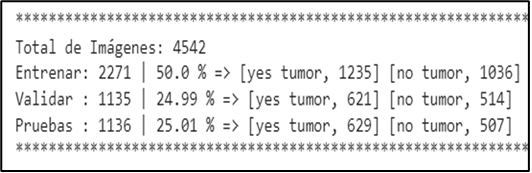
\includegraphics[scale=0.52]{figuras/fig1.png}
	\captionof{figure}{Estadística de datos a ser usados por el modelo.}\label{figura1}
\end{figura}

Evaluando la metadata de las imágenes se puede apreciar que no disponen un estándar en la dimensión de las imágenes, se realiza el redimensionamiento de estas a 224 de width y 224 de height.

\begin{figura}%[htb]
	\centering
	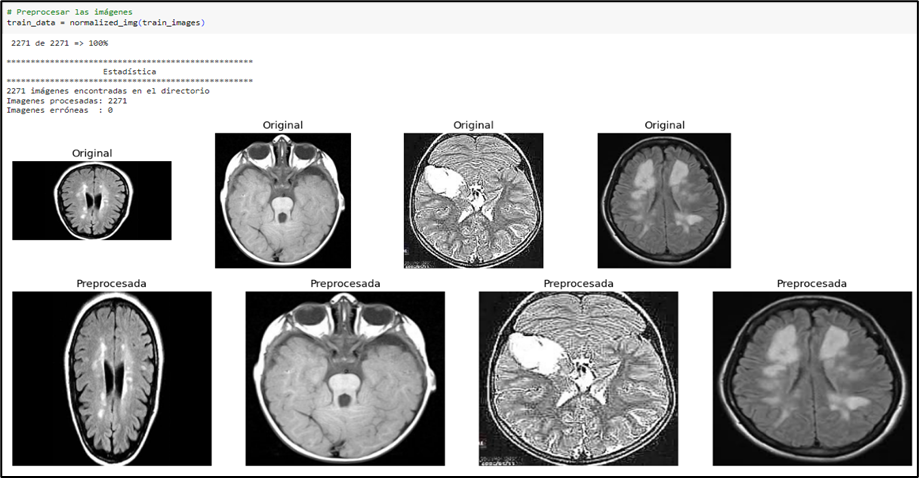
\includegraphics[scale=0.3]{figuras/fig2.png}
	\captionof{figure}{Resumen de procesamiento de imágenes por redimensionamiento.}
	\label{figura2}
\end{figura}

\subsection{Modelo}
Dentro de los paquetes de tensorflow se puede importar la red del modelo para VGGNet16, sin embargo, hay que hacer los ajustes de entrada y salida dependiendo del tipo de clasificación que se use. 
A continuación, se muestra las librerías usadas para el entrenamiento del modelo.

\begin{figura}%[htb]
	\centering
	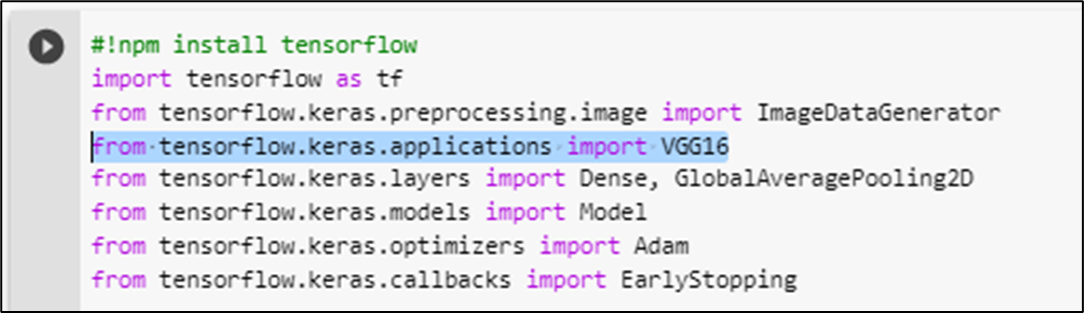
\includegraphics[scale=0.24]{figuras/fig3.png}
	\captionof{figure}{Paquetes o librerías usadas.}
	\label{figura3}
\end{figura}

Para el estudio se plantea un caso de clasificación binaria por lo cual la última capa corresponde a \texttt{sigmoid} y al compilar el modelo se establece la perdida como \texttt{binary\_crossentropy}.

\begin{figura}%[htb]
	\centering
	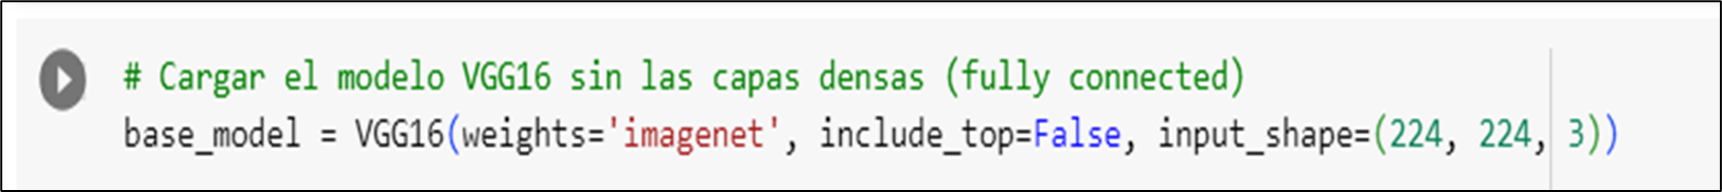
\includegraphics[scale=0.17]{figuras/fig4.png}
	\captionof{figure}{Modelo VGG16.}
	\label{figura4}
\end{figura}

\begin{figura}%[htb]
	\centering
	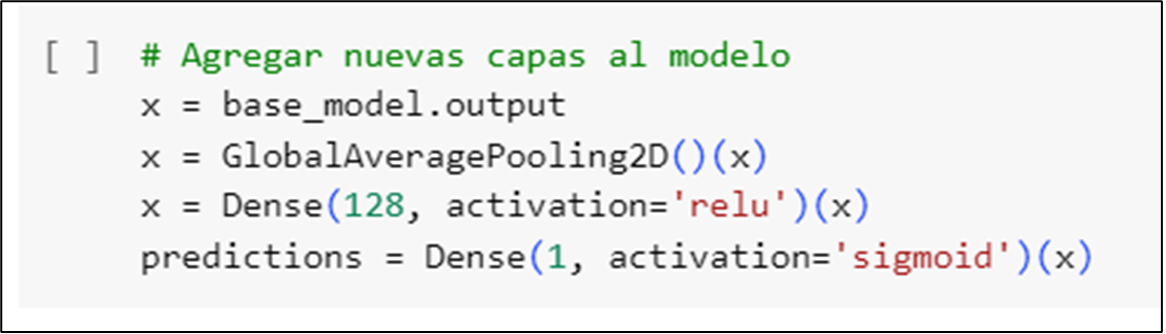
\includegraphics[scale=0.24]{figuras/fig5.png}
	\captionof{figure}{Nuevas capas al modelo, se establece la salida binara.}
	\label{figura5}
\end{figura}

\begin{figura}%[htb]
	\centering
	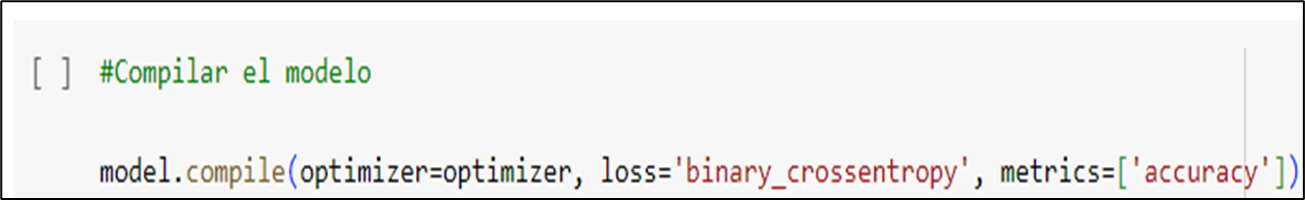
\includegraphics[scale=0.22]{figuras/fig6.png}
	\captionof{figure}{Modelo compilado para clasificación binaria.}
	\label{figura6}
\end{figura}


\subsection{Ajustes en el entrenamiento}
Se estableció los siguientes parámetros:
\begin{itemize}
	\item \texttt{Learning Rate Schedule = 0.0001}	
	\item \texttt{Epochs = 100}
	\item \texttt{EarlyStopping => (monitor='val\_loss', patience=5, verbose=1, \\ restore\_best\_weights=True)}
\end{itemize}

\subsubsection{Modelo VGGNet16 con clasificación binaria}
\begin{figura}%[htb]
	\centering
	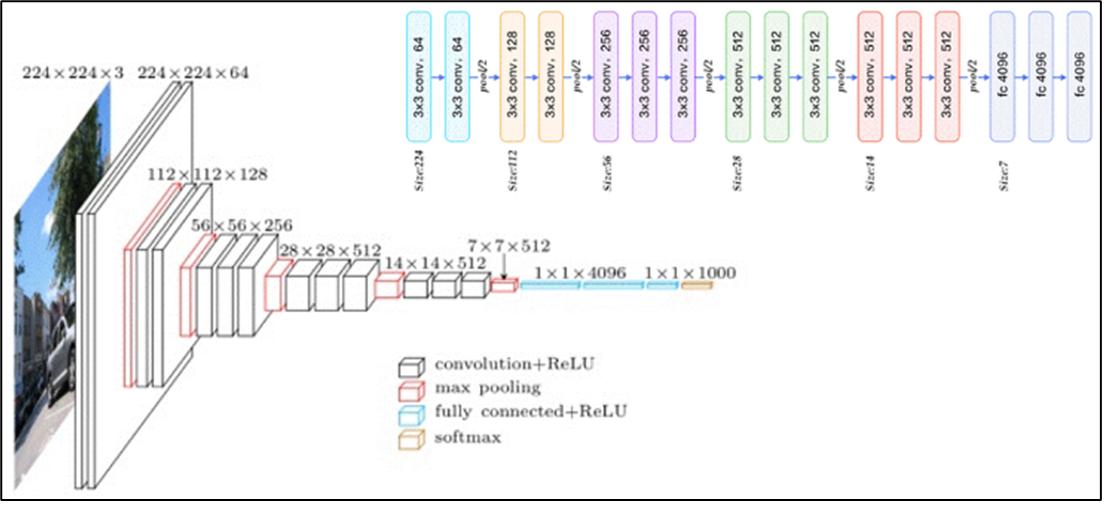
\includegraphics[scale=0.25]{figuras/fig7.png}
	\captionof{figure}{Arquitectura VGGNet 16, explicación gráfica.}
	\label{figura7}
\end{figura}


\begin{figura}%[htb]
	\centering
	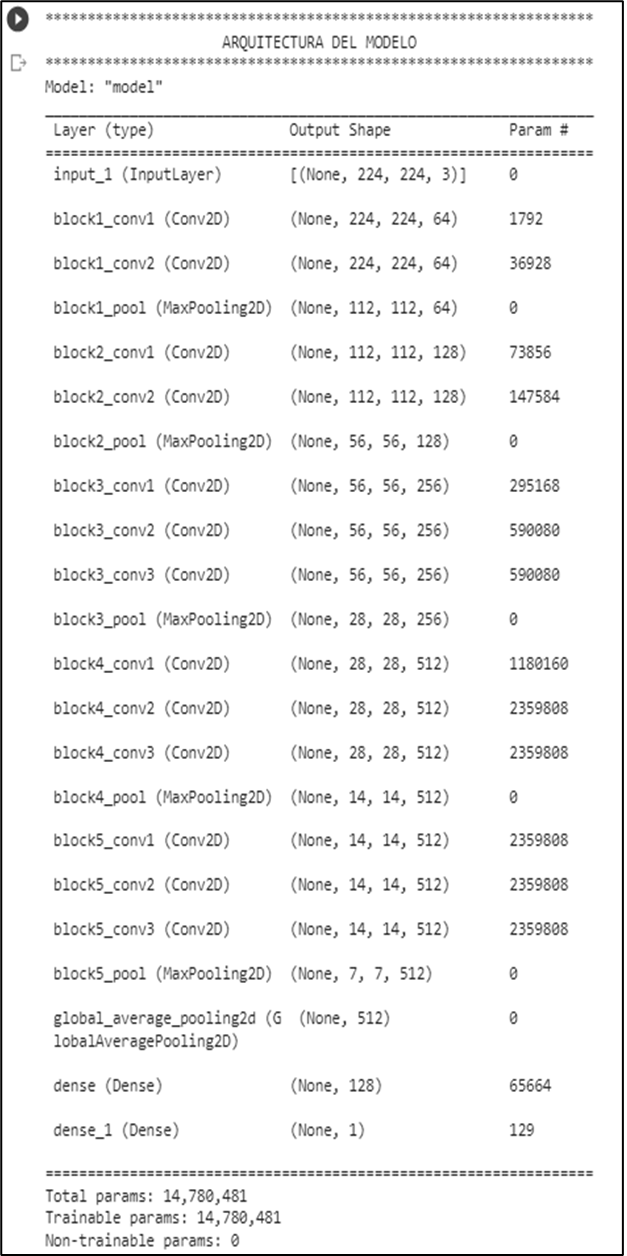
\includegraphics[scale=0.45]{figuras/fig8.png}
	\captionof{figure}{Arquitectura VGGNet 16, vista de la arquitectura del modelo configurado.}
	\label{figura8}
\end{figura}


%Las secciones de Introducción, Materiales y Métodos, Resultados, Discusión y Conclusiones del artículo pueden estructurarse divididas en diferente forma. Si el artículo describe un estudio efectuado en un área en particular, esta debe ser escrita en subencabezamientos bajo Materiales y Métodos. En esta plantilla en la sección materiales y métodos se explica cada una de las partes del manuscrito y como elaborarlo.
%
%\subsection{Configuración de página}
%
%El contenido del artículo debe ser redactado en un tamaño de página tipo carta (21 x 28 cm). Los márgenes deben ser: superior e inferior de 25mm, izquierdo y derecho 20 mm. La hoja debe estar dividida en dos columnas con un espacio de 5.1 mm entre las columnas. Todos los párrafos deben tener tabulaciones en la primera línea, menos el primero luego del subtítulo correspondiente y el texto debe estar justificado totalmente. 
%      La versión final del artículo se debe enviar en un archivo en formato PDF con el fin de publicarlo en línea y en formato Word para su publicación impresa.
%
%\subsection{Título principal}
%
%El título principal (en la primera página) debe estar centrado y con fuente Times New Roman tamaño 18, escrito con letras mayúsculas y con la primera letra de las palabras mayores en mayor tamaño
%
%\subsection{Nombre del Autor(s) y afiliaciones}
%
%Los nombres del autor(es) deben estar centrados abajo del título y con fuente Times New Roman tamaño 10, sin negrita tal como se indica en la parte superior de este documento.
%      Se escribirá primero el nombre y luego el apellido. En el caso de que el artículo tenga más de un autor, los nombres estarán separados por comas de manera que todos los nombres se los autores estén en una sola línea. Los detalles de los autores no deben mostrar ningún título profesional como PhD, MSc, Dr.
%
%\subsection{Títulos de primer orden}
%
%El primer nivel corresponde al de título, por tanto debe estar alineado a la izquierda, indexado con números arábigos con la primera letra en mayúscula  y todas las demás letras en minúscula. Debe presentarse con fuente Times New Roman tamaño 15 con el estilo título. Use un punto (".") después del número del título. 
%
%\subsection{Títulos de segundo y tercer orden}
%
%Un segundo nivel corresponde al subtítulo y es como el que está leyendo. Estos títulos deben estar en negrita con Times New  Roman en tamaño 13. La primera letra debe estar en mayúscula, con alineación a la izquierda como en este párrafo. Para los títulos de tercer orden utilice la fuente Times New Roman tipo cursiva en tamaño 12, enlistado con números arábigos seguidos por un paréntesis 1), 2), etc. La primera letra debe estar con letra mayúscula, con alineación a la izquierda y el texto del ítem debe estar inmediatamente después del encabezado sin saltos de línea.
%
%\subsection{Texto principal}
%
%Escriba el texto principal con la fuente Times New Roman tamaño 12, espaciado sencillo. No utilice doble espacio. Todos los párrafos deben tener la primera línea con la tabulación de esta guía y no se debe adicionar ninguna línea en blanco entre los párrafos. El texto deberá estar totalmente justificado.
%
%\subsection{Figuras, tablas, ecuaciones, unidades y abreviaturas.}
%
%1) Figuras: Todas las figuras deben estar centradas en la columna y colocadas en el recuadro indicado en esta guía y guardadasenla carpeta Figuras. En la figura 1 se muestra un ejemplo del cómo se debe presentar las figuras en el artículo. 
%El título de la figura se coloca en la parte inferior de la misma y debe ser con fuente Times New Roman, tamaño 9 sin negrita. 
%El nombre de la figura debe tener mayúscula solamente en la primera palabra, independientemente de si se trata de una palabra mayor o menor. El nombre de la figura se utiliza centrado en la columna, si la descripción se extiende más de una línea el texto se debe mostrar de forma justificada.
%
%\begin{figura}%[htb]
%\centering
%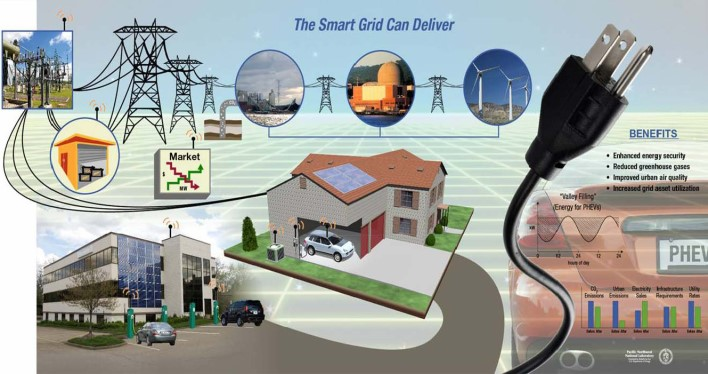
\includegraphics[scale=1]{figuras/fig1}
%\captionof{figure}{Nombre de la Figura.\cite{1}}\label{figura1}
%\end{figura}
%
%En el nombre  para indicar se escribe “Figura” y un número de secuencia Figura 1. , Figura 2. , etc.; deben seguir dos espacios para colocar el título.   La figura debe tratar de colocarse en la parte superior o inferior de cada columna. Una figura grande puede colocarse en la parte superior o inferior de la página y ocupar el espacio de dos columnas pero no deberán sobrepasar los márgenes. Si la figura posee dos partes incluya los indicativos “(a)” y “(b)” en la parte inferior de cada gráfico. Debe verificar que las figuras que se encuentren en el artículo se citen en el texto principal.
%
%     Proporcione las ilustraciones a color o en blanco y negro con una resolución adecuada (300 dpi) de manera que la figura se pueda apreciar con claridad en el documento. No utilice figuras de baja resolución porque empobrece la calidad del artículo. 
%2) Tablas: Coloque las tablas al inicio o al final de las columnas. El título de las tablas se coloca en la parte superior de la misma con fuente Times New Roman tamaño 9 con la primera letra mayúscula (estilo título), centrado en la columna, sin negrita. Antes de la línea del título, se incluye una línea centrada donde se usa la palabra “Tabla” seguida de la numeración de la tabla usando números arábigos.
%
%El texto de la tabla debe estar con fuente Times New Roman tamaño 9 sin negrita. La Tabla 1 de esta guía es un ejemplo del formato para la presentación del artículo.
%
%\begin{tabla}%[htbp]
%  \centering
%  \captionof{table}{Tamaños de Fuente Times New Roman y  Estilos Empleados en la revista INGENIUS}
%  \scalebox{0.74}{
%    \begin{tabular}{cl}
%    \toprule
%    \multicolumn{1}{c}{Tamaño de letra} & \multicolumn{1}{c}{Uso} \\
%    \midrule
%    \small{10}    & \small{Datos del autor, título, texto de tablas y figuras.} \\
%    \textit{\textbf{12}} & \textbf{Resumen, palabras clave} \\
%    12    & Nombre del autor(es), texto del artículo  \\
%    \Large{13}    & \Large{Títulos de segundo y tercer orden} \\
%    \LARGE{\textbf{15}} & \LARGE{\textbf{Títulos de primer nivel}} \\
%    \huge{\textbf{18}} & \huge{\textbf{TITULO}} \\
%    \bottomrule
%    \end{tabular}%
%}
%  \label{tabla1}%
%\end{tabla}%
%Debe verificar que las tablas que se encuentren en el artículo se citen en el texto principal. 
%
%3)  Ecuaciones: Utilice el editor de ecuaciones de Microsoft Word.  Trate de que las ecuaciones sean compactas empleando en el signo (/), la función exponencial como exp, o subíndices y superíndices. Enumere las ecuaciones consecutivamente colocando la numeración entre paréntesis y alineándola con el margen derecho. La ecuación debe estar centrada. 
%
%\begin{equation}\label{eq3}
%(1 + x)^{n} = 1 + \frac{nx}{1!} + \frac{n(n-1)x^{2}}{2!} + \cdots
%\end{equation}
%
%4) Unidades: Las unidades recomendadas son las del sistema métrico, en particular, se sugiere el uso del Sistema Internacional de Unidades (Unidades SI). Las unidades del sistema inglés pueden emplearse como unidades secundarias (en paréntesis). 
%5) Abreviaturas:
%Se deben definir las abreviaturas y acrónimos que no sean comunes la primera vez que aparecen en el texto, aún si ya se han definido en el resumen. Abre. No utilice abreviaturas en el título a menos que sea inevitable.
%
%\subsection{Referencias}
%
%Se debe verificar con cuidado que todas las citas colocadas en el texto, aparezcan en la lista de referencias bibliográficas. En la lista solo deben aparecer las referencias que fueron utilizadas en el texto principal del trabajo, en las tablas o en las figuras, esto implica que no deben aparecer otras referencias aunque el autor las haya consultado durante la preparación del artículo.
%        Las referencias incluidas en el texto se presentan al final ordenadas numéricamente en paréntesis cuadrados \cite{2} según el orden de aparición en el texto. Un punto debe seguir al paréntesis \cite{3}. Referencias múltiples pueden citarse con paréntesis separados por un guión \cite{1,2,3}. Cuando se cite un libro indicar las páginas con la información relevante. El título como tal de las “Referencias” al final del artículo no va numerado.
%Al final del artículo liste y enumere todas las referencias bibliográficas con una fuente Times New Roman tamaño 12. Proporcione todos los nombres de los autores; use “et al” si hay seis autores o más.  Los nombres de persona deben abreviarse poniendo sólo las iniciales Se debe verificar con cuidado que todas las citas colocadas en el texto aparezcan en la lista de referencias bibliográficas.
%      En la lista sólo deben aparecer las referencias que fueron utilizadas en el texto principal del trabajo, en las tablas o en las figuras, esto implica que no deben aparecer otras referencias aunque el autor las haya consultado durante la preparación del artículo.
%Puede consultar la guía del IEEE para la cita de referencias disponible en el link http://www.ieee.org/documents/ieeecitationref.pdf
%
%      En la sección  “Referencias” se presenta formatos para diferentes tipos de citas siguiendo lo que indica el formato IEEE. No use los subtitulos, únicamente coloque las refrencias en orden de aparición en el texto de acuerdo a lo que corresponda.
%
%Las referencias deben ser guardadas en el archivo \textbf{bib\_plantilla} en formato bibtex, indicando la \textbf{bibkey} secuencialmente según su aparición, se recomienda utilizar \textbf{JABREF}

\section{Resultados y Discusión}

%Estos dos apartados suelen aparecer juntos en muchos trabajos. No debemos confundir esta discusión o análisis con la obtención de conclusiones, algo que depende tanto de los resultados y de su análisis como del marco teórico y de los objetivos.

Una vez entrenado el modelo con el marco establecido en el capítulo anterior, se obtiene corte en epoch 23 por tener activo \texttt{EarlyStopping} en la métrica de \texttt{val\_loss}, con esto se evita un sobre aprendizaje del modelo; es decir, cuando el valor de la perdida es constante y no sufre cambios consecutivos, el modelo deja de aprender porque llegó a su máximo en epoch 18 y EarlyStopping hace que se termine el proceso. 

\begin{figura}%[htb]
\centering
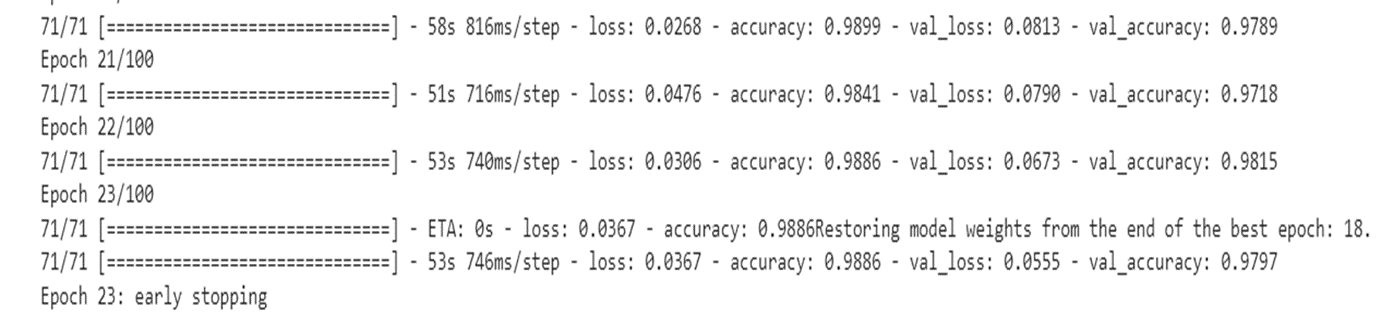
\includegraphics[scale=0.22]{figuras/fig9.png}
\captionof{figure}{Histórico de entrenamiento del modelo.\cite{1}}\label{figura9}
\end{figura}

\subsection{Validación}
En la evaluación del modelo con el segmento de imágenes para pruebas se pudo llegar a una pérdida de 3.92\% y una exactitud del 98.68\% siendo buenos rangos para la predicción.\\
A continuación, se muestra los histogramas para la perdida y precisión:

\begin{figura}%[htb]
	\centering
	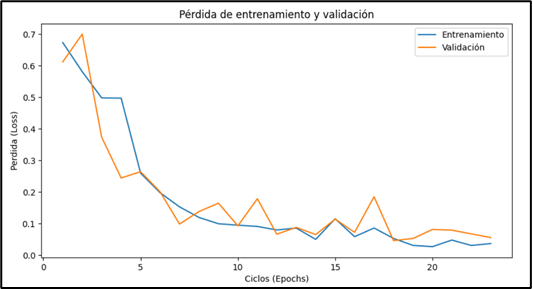
\includegraphics[scale=0.5]{figuras/fig10.png}
	\captionof{figure}{Histograma de pérdida.\cite{1}}\label{figura10}
\end{figura}

\begin{figura}%[htb]
	\centering
	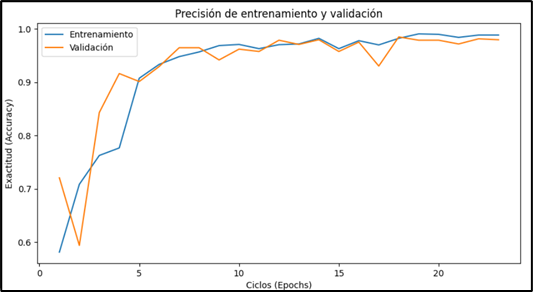
\includegraphics[scale=0.5]{figuras/fig11.png}
	\captionof{figure}{Histograma de precisión.\cite{1}}\label{figura11}
\end{figura}

\subsection{Predicción}
Culminada las fases anteriores se dispone de un modelo entrenado y dispuesto a dar predicciones con una exactitud del 98\%, esto quiere decir que es capaz de identificar si existe o no tumor en una RX Cerebral.\\
Para validar lo dicho se toma las 58 imágenes separadas al inicio del ejercicio, el modelo las recibe para predecir si tienen o no tumor, al final se hace una comparación con la matriz del archivo csv el cual contiene datos clasificatorios previos.\\
A continuación, se muestra gráfica de la curva ROC la cual nos muestra el resultado de la exactitud predicción realizada en estas 58 imágenes.

\begin{figura}%[htb]
	\centering
	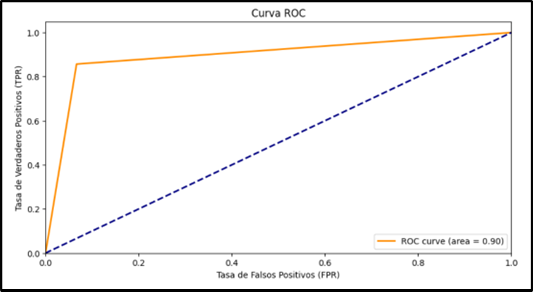
\includegraphics[scale=0.5]{figuras/fig12.png}
	\captionof{figure}{Histograma curva ROC.\cite{1}}\label{figura12}
\end{figura}

Según el estudio realizado en 2020 por Ejaz Ul Haq, Huang Jianjun, Kang Li, Hafeez Ul Haq \& Tijiang Zhang ("An MRI-based deep learning approach for efficient classification of brain tumors") \cite{17} el cual se centró en la detección y diagnóstico de tumores cerebrales utilizando escaneos de resonancia magnética (MRI ) y redes neuronales convolucionales, los autores exploraron la capacidad de las redes neuronales para identificar patrones sutiles en las imágenes de MRI, los resultados experimentales demuestran una precisión del 97,3\% y un coeficiente de similitud de dados (DSC ) del 95,8\% en la tarea de clasificar el tumor cerebral como gliomas, meningiomas o tumores hipofisarios logrados por la primera arquitectura CNN propuesta, mientras que la segunda arquitectura CNN propuesta logró una precisión del 96,5\% con un DSC del 94,3\% en la tarea de clasificar los grados de glioma como HGG  o LGG . \\

Como se muestra en el estudio, basados en artículos científicos similares con alto grado de precisión, hemos planteado un caso con un segmento de imágenes de RX Cerebrales clasificados por tumorales y no tumorales; como VGGNet-16 se caracteriza por tener una arquitectura profunda y compleja, argumentada por 16 capas convolucionales y 3 capas totalmente conectadas. Estas capas facilitan a extraer características de las imágenes, mientras que las 3 capas son usadas para la clasificación. 
A lo largo de las etapas, se tomaron decisiones y ajustes clave que contribuyeron al éxito del modelo.
\begin{itemize}
	\item Selección y Preprocesamiento de Datos: Se utilizó el dataset Brain Tumor Dataset, que contenía imágenes de radiografías cerebrales clasificadas en "Tumor" y "Healthy". Se llevó a cabo una selección aleatoria de imágenes para la evaluación y se creó un archivo CSV para respaldar esta selección. Las imágenes se redimensionaron a un tamaño uniforme de 224x224 píxeles para garantizar la entrada consistente al modelo.
	\item Arquitectura del Modelo VGGNet16: La arquitectura VGGNet16, conocida por su simplicidad y profundidad, se utilizó como base. La última capa de clasificación se adaptó para la clasificación binaria utilizando una función de activación sigmoid y la pérdida se estableció como binary\_crossentropy. Se configuró un Learning Rate Schedule y se aplicó EarlyStopping para evitar el sobreaprendizaje.
	\item Entrenamiento y Evaluación del Modelo: El modelo se entrenó en un total de 100 epochs, pero se utilizó EarlyStopping para finalizar el proceso en el epoch 23 debido a que la métrica de val\_loss dejó de mejorar. Se logró una pérdida del 3.92\% y una exactitud del 98.68\% en la evaluación del conjunto de pruebas, indicando un alto rendimiento en la predicción de imágenes cerebrales.
\end{itemize}

\subsection{Análisis Comparativo}
Tanto el presente estudio como el estudio de MRI lograron altos niveles de precisión en la predicción de tumores cerebrales, con un 98.68\% y un 97.3\% respectivamente. Esto indica que ambas metodologías y enfoques de entrenamiento son efectivos en la detección de patologías cerebrales.\\

Ambos estudios optaron por utilizar la arquitectura VGGNet16, lo que sugiere que esta arquitectura en particular ha demostrado ser eficaz en la clasificación de imágenes médicas. Sin embargo, el estudio de MRI pudo haber realizado ajustes específicos en la estructura de la red o en los hiperparámetros para optimizar aún más el rendimiento.\\

El estudio de MRI utilizó un conjunto de datos similar en tamaño al mostrado en el documento, con 3062 imágenes en total. Esto demuestra que un conjunto de datos suficientemente grande puede ser crucial para el éxito de la red neuronal en la detección de patologías.\\

El estudio de MRI destacó la validación clínica exhaustiva en un entorno médico real, lo que sugiere un enfoque más completo para evaluar la eficacia del modelo. Esto puede ser especialmente importante en la adopción del modelo en la práctica médica.\\

La colaboración con expertos en radiología en el estudio de MRI podría haber aportado conocimientos médicos adicionales y contribuido a la mejora del modelo. La combinación de experiencia clínica y capacidades de IA es una tendencia en auge en la investigación médica.\\

Ambos estudios podrían mencionar la necesidad de mantener el modelo actualizado en función de las cambiantes prácticas médicas y los avances tecnológicos en el campo de la imagenología.\\

En última instancia, el análisis comparativo destaca la similitud en los enfoques y logros entre los dos estudios, lo que sugiere que la detección de tumores cerebrales utilizando redes neuronales convolucionales es un campo en desarrollo con enfoques comunes y resultados prometedores. Sin embargo, las diferencias en aspectos como la validación clínica y la colaboración con expertos pueden influir en la confiabilidad y aplicabilidad del modelo en un entorno médico real.\\

Aunque el estudio ha demostrado resultados prometedores en la detección de tumores cerebrales utilizando redes neuronales convolucionales (CNN) con la arquitectura VGGNet16, también es importante tener en cuenta las limitaciones que podrían afectar la generalización y aplicabilidad del modelo en un entorno clínico:
\begin{itemize}
	\item Tamaño y Diversidad del Conjunto de Datos: El tamaño del conjunto de datos utilizado puede afectar la capacidad del modelo para generalizar de manera efectiva a casos no vistos. Además, la diversidad de las imágenes en términos de género, edad, etnia y otras características demográficas puede influir en la capacidad del modelo para adaptarse a diferentes poblaciones.
	\item Variabilidad de las Imágenes: Las imágenes médicas pueden variar en calidad, iluminación, posición del paciente y artefactos. Si el modelo no se entrena con una amplia variedad de condiciones, podría tener dificultades para manejar estas variabilidades en un entorno clínico real.
	\item Sobreaprendizaje (Overfitting): Aunque el EarlyStopping se utilizó para evitar el sobreaprendizaje durante el entrenamiento, es posible que el modelo todavía haya memorizado características específicas del conjunto de datos de entrenamiento y no generalice bien a datos nuevos. Esto podría ser especialmente relevante si el conjunto de datos no es lo suficientemente grande o diverso.
	\item Interpretabilidad del Modelo: Las CNN, especialmente modelos profundos como VGGNet16, pueden ser inherentemente difíciles de interpretar. Esto puede ser un desafío en un entorno médico donde los médicos necesitan entender y justificar las decisiones tomadas por el modelo.
	\item Etiquetado de Datos: La precisión de las etiquetas de las imágenes en el conjunto de datos es crucial. Si hay errores en las etiquetas o si las imágenes se clasificaron incorrectamente, el rendimiento del modelo podría verse afectado.
	\item Limitaciones Éticas y Legales: La implementación de un modelo de diagnóstico automatizado en un entorno clínico plantea cuestiones éticas y legales. Los médicos deben ser cautelosos al confiar completamente en un modelo sin la supervisión humana adecuada.
	\item Heterogeneidad de Tumores: Los tumores cerebrales pueden variar en tipo, tamaño, forma y ubicación. El modelo podría tener dificultades para detectar tumores menos comunes o con características atípicas.
	\item Sensibilidad a Cambios en los Protocolos de Imagen: Los protocolos de adquisición de imágenes pueden variar entre instituciones médicas y con el tiempo. El modelo puede no rendir tan bien si se presenta con imágenes adquiridas con protocolos diferentes a los utilizados en el conjunto de datos de entrenamiento.
	\item Necesidad de Validación Clínica: Aunque el modelo tiene un alto rendimiento en términos de métricas de evaluación, es esencial realizar estudios clínicos y validaciones en un entorno médico real antes de implementar el modelo en la práctica clínica.
	\item Actualización Continua: Los modelos de IA, incluidas las CNN, pueden volverse obsoletos con el tiempo debido a avances tecnológicos y cambios en la adquisición de imágenes y protocolos clínicos. El modelo requerirá una actualización constante para mantener su precisión y relevancia.
\end{itemize}

Si bien las redes neuronales convolucionales y la arquitectura VGGNet16 ofrecen avances significativos en el análisis de imágenes médicas, es fundamental considerar estas limitaciones y desafíos para garantizar un despliegue efectivo y seguro en un entorno clínico.


\section{Conclusiones}

%Las conclusiones deben obtenerse, por tanto, a partir de algo más que de los simples datos registrados. De hecho, unos datos o resultados pueden tener un sentido u otro y, por tanto, pueden llevarnos a unas conclusiones y otras, dependiendo del marco conceptual que justifica nuestra investigación, de la metodología seguida, de los objetivos propuestos, etc.

El estudio demuestra la eficacia de la arquitectura VGGNet16 en la clasificación de imágenes de radiografías cerebrales con y sin tumor cerebral. Las siguientes conclusiones se pueden derivar de los resultados y el proceso llevado a cabo:
\begin{itemize}
	\item Potencial de las CNN en Imágenes Médicas: La utilización de redes neuronales convolucionales, en particular VGGNet16, ha demostrado su potencial para mejorar la precisión y eficiencia en el diagnóstico radiológico de patologías cerebrales. La capacidad de aprender representaciones jerárquicas de las imágenes resulta valiosa en la detección de patrones y estructuras complejas.
	\item Importancia del preprocesamiento: El preprocesamiento adecuado de las imágenes es esencial para garantizar que el modelo reciba datos coherentes y relevantes. La normalización, eliminación de artefactos y redimensionamiento de las imágenes contribuyeron al rendimiento del modelo.
	\item Ajustes de Hiperparámetros: La elección adecuada de hiperparámetros, como el Learning Rate Schedule y EarlyStopping, es crucial para un entrenamiento eficaz y para evitar el sobreaprendizaje del modelo.
	\item Alto Rendimiento del Modelo: El modelo entrenado alcanzó una alta exactitud del 98.68\% en la predicción de imágenes de prueba, lo que sugiere que es capaz de identificar la presencia de un tumor cerebral en una radiografía cerebral con un alto grado de certeza.
	\item Validación y Aplicación Clínica: La validación del modelo utilizando el conjunto de imágenes separadas al comienzo del estudio y la comparación con la matriz del archivo CSV respaldan la capacidad del modelo para realizar predicciones precisas. Esto podría tener aplicaciones clínicas valiosas como una herramienta de apoyo para radiólogos en la detección temprana de tumores cerebrales.
\end{itemize}

El estudio demuestra que la combinación de la arquitectura VGGNet16, técnicas de preprocesamiento y ajustes cuidadosos de hiperparámetros puede resultar en un modelo de CNN altamente preciso para la detección de tumores cerebrales en imágenes de radiografías. Los resultados respaldan la viabilidad de esta metodología en la práctica médica y resaltan el papel prometedor de la inteligencia artificial en el campo de la radiología.


\bibliography{bib_plantilla}
%\balance
\bibliographystyle{IEEEtran}
%}
\end{multicols}

%\begin{figure*}[htb]
%        \centering
% \begin{subfigure}[b]{0.33\textwidth}
% \centering
%              \includegraphics[scale=0.4]{figures/main}
%                \caption{Main menu} \label{fig:main}
%        \end{subfigure}%
%     \centering
%     \begin{subfigure}[b]{0.33\textwidth}
% \centering
%          \includegraphics[scale=0.4]{figures/loja}
%                \caption{Scenario 1: Downtown Loja}\label{fig:loja}
%        \end{subfigure}
%     \begin{subfigure}[b]{0.33\textwidth}
% \centering
%          \includegraphics[scale=0.4]{figures/utpl}
%                \caption{Scenario 2: UTPL Campus}\label{fig:utpl}
%        \end{subfigure}
%             \caption{Data visualization. }\label{figura1}
%\end{figure*}

\end{document}